%! TEX root = meet7.tex
% the main TeX file which is intended to compile, :VimtexReload after adjustment
% :h vimtex-tex-root
\documentclass[../main.tex]{subfiles}
% \includeonlyframes{two}
\setbeameroption{hide notes} % Only slides
% \setbeameroption{show only notes} % Only notes
% \setbeameroption{show notes on second screen=right} % Both

\begin{document}

\begin{frame}[t,mybg=bg3,mytitle=standard,light]%rmve mycolor when use mybg\\labelonfirst
	\frametitle{Univariat inferensial}
	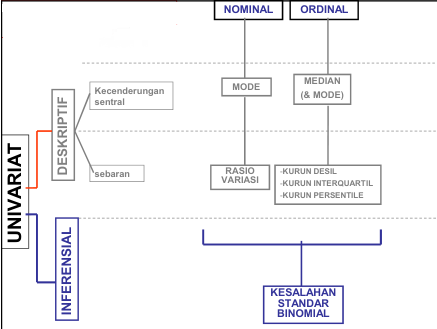
\includegraphics[width=.9\textwidth]{7inf1}

\end{frame}

\begin{frame}[t,mybg=placeholder,mytitle=standard,mycolor=digiPH_leaf,light]%rmve mycolor when use mybg\\labelonfirst
	\frametitle{Univariat inferensial}
	\framesubtitle{nominal dan ordinal}

	\onslide<1->{\boxes{digiPH_ocean}{white}{Pengertian: menarik kesimpulan tentang populasi berdasar kesimpulan pola data sampel.}}

	\onslide<2->{\boxes{green}{white}{Bila diambil sampel berkali-kali maka \textsf{mode} sampel-sampel akan terlihat mode populasi.}

		\begin{columns}
			\begin{column}{0.5\textwidth}
				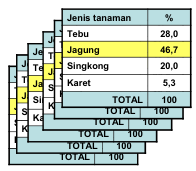
\includegraphics[width=34mm]{7inf2}
			\end{column}
			\begin{column}{0.5\textwidth}
				\boldblue{ -> Menarik kesimpulan populasi  }
			\end{column}
		\end{columns}}
\end{frame}

\begin{frame}[t,mybg=bg,mytitle=standard,light]%rmve mycolor when use mybg\\labelonfirst
	\frametitle{Univariat inferensial}
	\framesubtitle{nominal dan ordinal}
	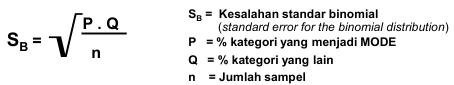
\includegraphics[width=.9\textwidth]{7inf3}

	\begin{columns}
		\begin{column}{0.4\textwidth}
			\only<2|handout:1>{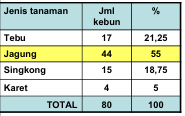
\includegraphics[width=40mm]{7tbl}\\}

			\only<3-|handout:2>{{\small Teori probabilitas menyatakan bahwa 95\% mode populasi akan berada $\pm$ 2 standard error of the sample mode.}}
		\end{column}
		\begin{column}{0.6\textwidth}
			\only<2|handout:1>{
				\begin{small}

					Contoh:\\
					Data jenis tanaman dengan n = 80\\
					Mode = jagung (55\%) = P\\ Q = 100-55\% = 45\%\\
					$ S_B =  \sqrt{ \frac{55.45}{80}} \to S_B = 5,56\%$\\
				\end{small}
			}


			\only<3-|handout:2>{\boldblue{Tempat kedudukan MODE Jagung pada POPULASI}

				= Mode $\pm$ 2 $S_B$\\ = 55\% $\pm$ 2 (5.56\%)

				= antara 43.88\% sampai dengan 66.12\%}

		\end{column}
	\end{columns}

\end{frame}

\begin{frame}[t,mybg=bg,mytitle=standard,light]%rmve mycolor when use mybg\\labelonfirst
	\frametitle{Analisis Deskriptif }
	\framesubtitle{Interval/rasio }
	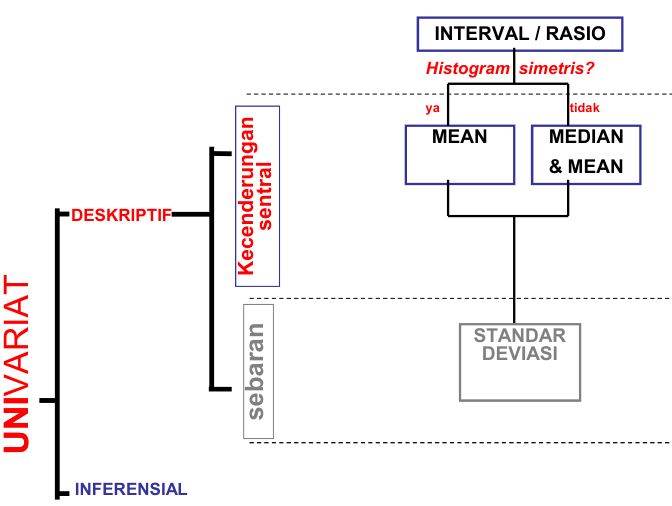
\includegraphics[width=.74\textwidth]{7inf4}
\end{frame}

\begin{frame}[label=two,t,mybg=bg,mytitle=standard,light]%rmve mycolor when use mybg\\labelonfirst
	\frametitle{Analisis Deskriptif }
	\framesubtitle{Interval/rasio }
	Contoh : berat badan mahasiswa  (n=11)
	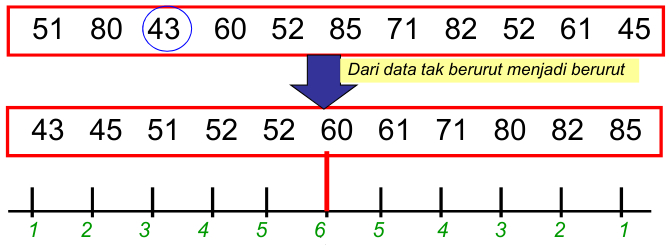
\includegraphics[width=.9\textwidth]{7inf5}
	{\small
		\begin{textblock*}{50mm}(50mm,70mm)
			\boxes{digiPH_red}{digiPH_black}{median = 60}
		\end{textblock*}}
	\vspace{3pt}
	{\small	\boxes{digiPH_red}{digiPH_black}{mean = (51+80+43+60+52+85+71+82+52+61+45) / 11 = 62}}

\end{frame}

\begin{frame}[label=two,t,mybg=bg,mytitle=standard,light]%rmve mycolor when use mybg\\labelonfirst
	\frametitle{Analisis Deskriptif }
	\framesubtitle{Interval/rasio }
	Contoh : berat badan mahasiswa  (n=10)
	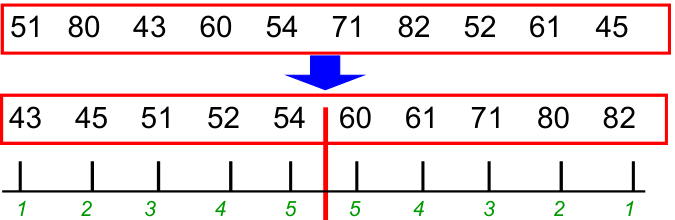
\includegraphics[width=.9\textwidth]{7inf6}
	{\small

		\begin{textblock*}{50mm}(50mm,70mm)
			\boxes{digiPH_red}{digiPH_black}{median = (54+60)/2 = 57}
		\end{textblock*}}
	\vspace{1cm}
	{\small	\boxes{digiPH_red}{digiPH_black}{mean =  (51+80+43+60+54+71+82+52+61+45) / 10 = 59,9}}

\end{frame}

\begin{frame}[t,mybg=bg,mytitle=standard,light]%rmve mycolor when use mybg\\labelonfirst
	\framesubtitle{Interval/rasio }

	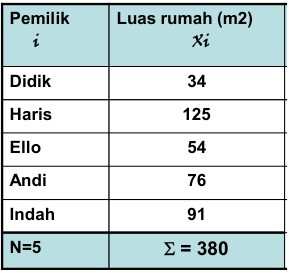
\includegraphics[width=40mm]{7mean}\\
	${\displaystyle A={\frac {1}{n}}\sum _{i=1}^{n}a_{i}={\frac {a_{1}+a_{2}+\cdots +a_{n}}{n}}}$\\
	$ = 380 / 5 $\\
	$ = 76$

\end{frame}

\begin{frame}[t,mybg=bg1,mytitle=standard,light]%rmve mycolor when use mybg\\labelonfirst
	\framesubtitle{Interval/rasio }
	\boldred{SEBARAN}

	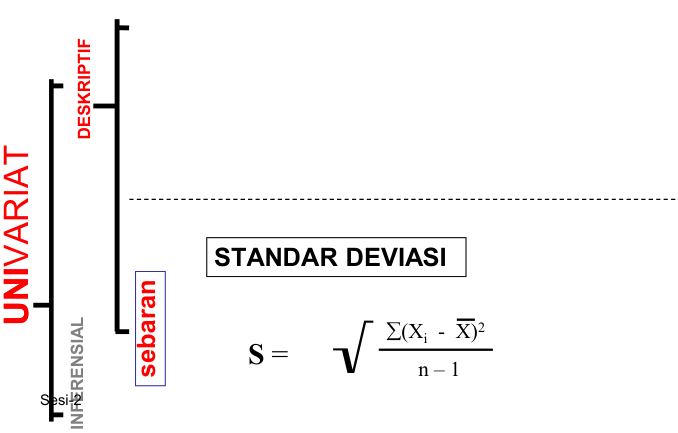
\includegraphics[width=.95\textwidth]{7mean2}
\end{frame}

\begin{frame}[t,mybg=bg,mytitle=standard,light]%rmve mycolor when use mybg\\labelonfirst
	\frametitle{`Asal Usul' Standar Deviasi}

	\only<1>{\begin{columns}
			\begin{column}{0.6\textwidth}

				mean deviation =  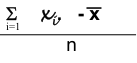
\includegraphics[width=27mm]{7for}

				MD = 60/6 = 10

			\end{column}
			\begin{column}{0.4\textwidth}
				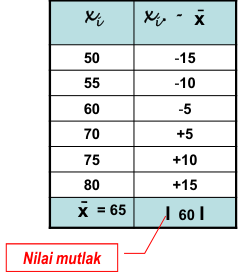
\includegraphics[width=.9\textwidth]{7mean3}
			\end{column}
		\end{columns}}

	\only<2->{Mean deviation adalah suatu ukuran sebaran yang baik,
		yang mencerminkan besarnya dispersi masing-masing
		data acak, hanya NILAI MUTLAK dalam matematika
		mempunyai sifat tidak baik -> \textcolor{red}{ jadi tidak dipakai !}

		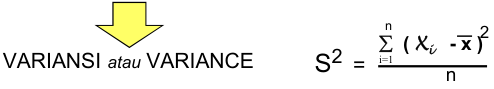
\includegraphics[width=.9\textwidth]{7var}}
	\only<3->{\begin{columns}
			\begin{column}{0.8\textwidth}
				Variansi adalah ukuran untuk dispersi yang baik yang mencerminkan besarnya tiap-tiap data acak, \textcolor{red}{tapi} punya kelemahan karena sifatnya yang \textcolor{red}{kuadrat}. Maka perlu diakar:
			\end{column}
			\begin{column}{0.2\textwidth}
				\boldred{-> Standard deviasi}
			\end{column}
		\end{columns}}



\end{frame}

\begin{frame}[t,mybg=bg,mytitle=standard,light]%rmve mycolor when use mybg\\labelonfirst
	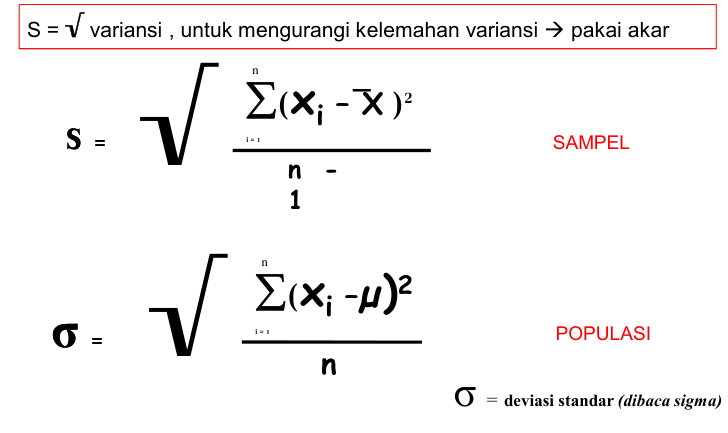
\includegraphics[width=.9\textwidth]{7var2}
\end{frame}

\begin{frame}[t,mybg=bg,mytitle=standard,light]%rmve mycolor when use mybg\\labelonfirst
	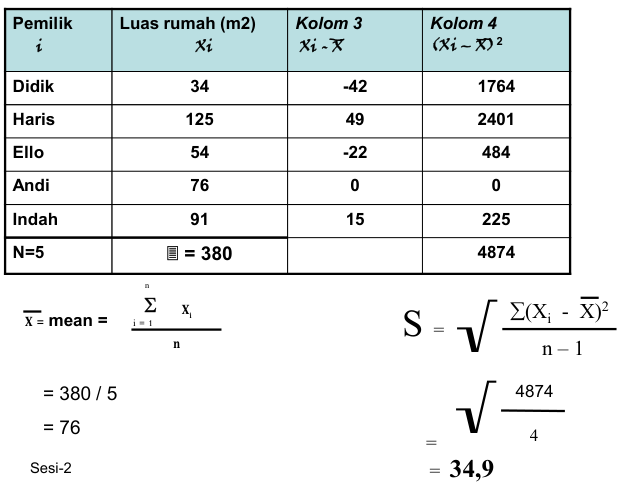
\includegraphics[width=.9\textwidth]{7var3}
\end{frame}

\begin{frame}[t,mybg=bg1,mytitle=standard,mycolor=digiPH_gray,light]%rmve mycolor when use mybg\\labelonfirst
	Cobalah dengan data dengan nilai sama

	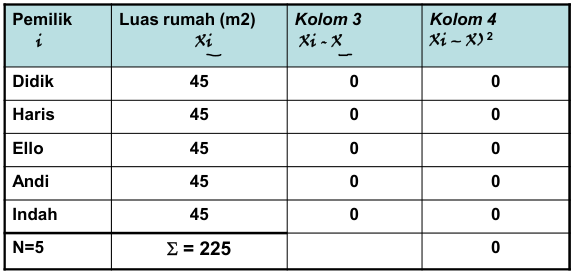
\includegraphics[width=80mm]{7var4}

	\begin{columns}
		\begin{column}{0.5\textwidth}
			$ \overline{x}=$ 225 / 5 \\
			\boldred{45}
		\end{column}
		\begin{column}{0.5\textwidth}
			S = 0
		\end{column}
	\end{columns}

	\boxes{digiPH_yellow}{digiPH_black}{Ini berarti tidak ada variasi dan semua data terpusat di nilai 45. Tidak ada sebaran karena standar deviasinya = 0}

\end{frame}








\end{document}
